\subsection{TEC-8总体结构}
本次计算机组成原理课程设计基于TEC-8实验台,TEC-8总体框架如图\ref{fig:construction_of_tec8}所示

\begin{figure}[H]
    \centering
    \label{fig:construction_of_tec8}
    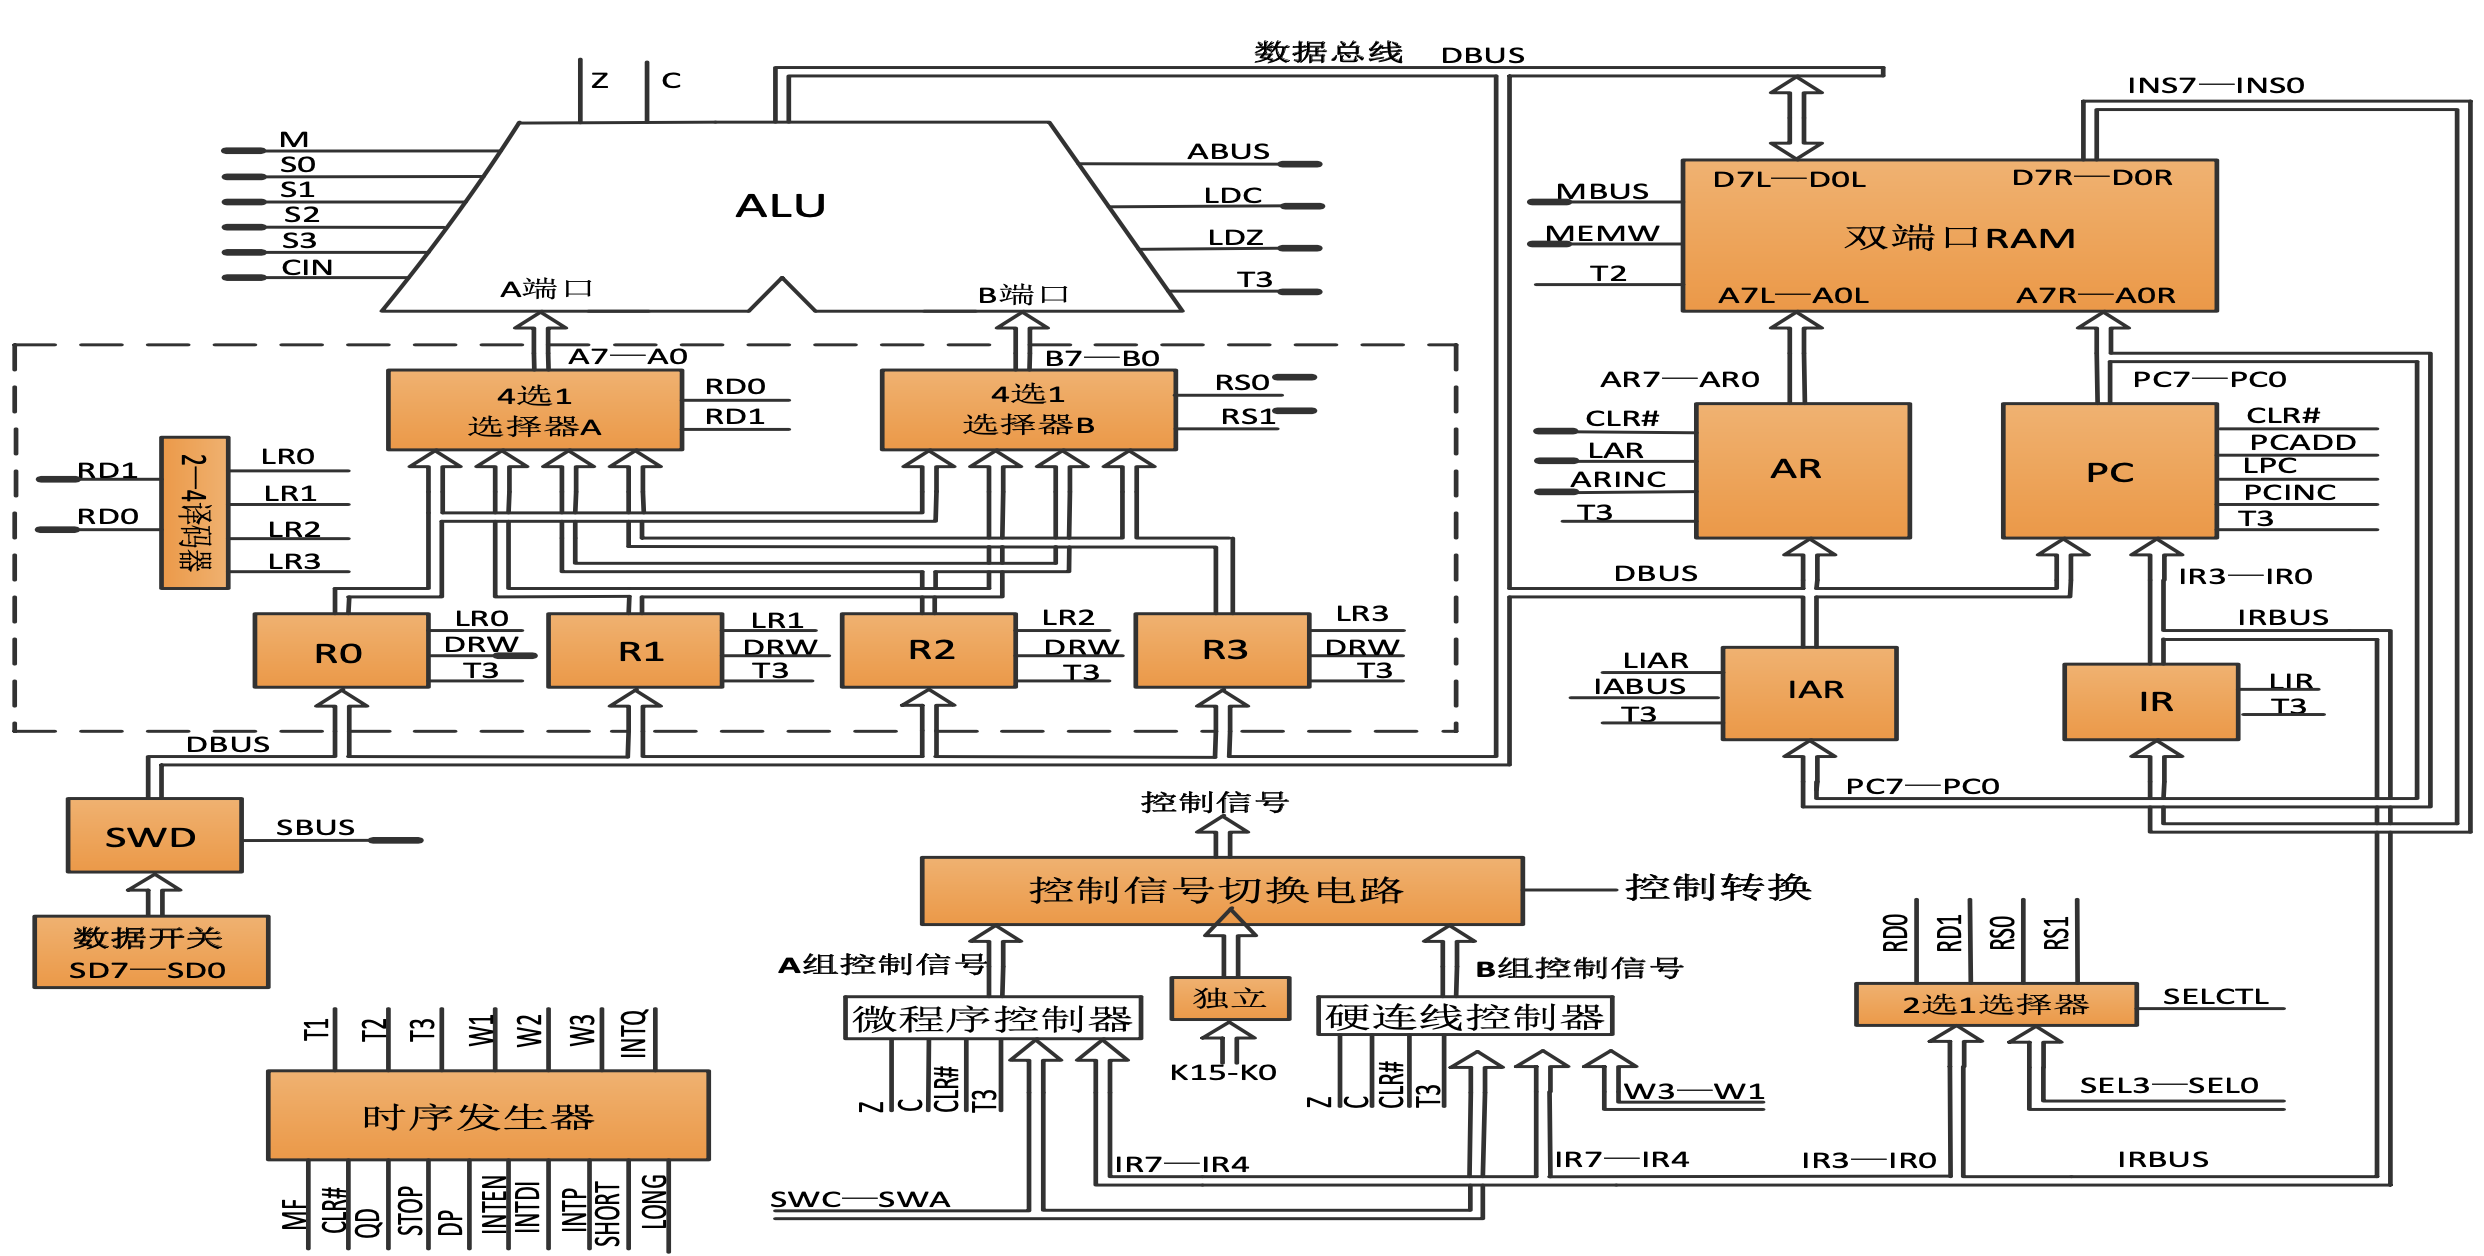
\includegraphics[width=0.9\textwidth]{figures/chapter1/QQ20220828-115423@2x.png}
    \caption{TEC-8结构图}
\end{figure}

其中各个信号的作用如表所示\ref{tab:output_signal}
\begin{table}[htbp]
    \label{tab:output_signal}
    \resizebox{0.9\linewidth}{!}{
    \begin{tabular}{|l|l|}
    \hline
    信号          & 说明                                                     \\ \hline
    CLR         & 复位                                                     \\ \hline
    T3          & 节拍脉冲                                                   \\ \hline
    SWCBA       & 控制台操作模式选择                                              \\ \hline
    IR7$\sim$4  & 指令寄存器高四位,标志指令类型                                        \\ \hline
    W3$\sim$W1  & 节拍电位信号                                                 \\ \hline
    C           & 进位标志                                                   \\ \hline
    Z           & 结果为0标志                                                 \\ \hline
    DRW         & =1时在T3上升沿,将数据总线中数据写入选中的寄存器                             \\ \hline
    LPC         & =1时在T3上升沿,将数据总线数据写入PC                                  \\ \hline
    PCINC       & =1时在T3上升沿将PC+1                                         \\ \hline
    LAR         & =1时在T3上升沿将数据总线数据写入AR                                   \\ \hline
    PCADD       & =1时在T3上升沿将PC的值加上IR3$\sim$1的值生成新的PC                     \\ \hline
    ARINC       & =1时在T3上升沿AR+1                                          \\ \hline
    SETCTL      & 见TEC-8结构图,SETCTL控制二选一选择器,\\设置RD0 RD1 RS0 RS1的值由IR还是SEL决定 \\ \hline
    MEMW        & =1时T2上升沿将数据总线上数据写入AR指定地址处                              \\ \hline
    STOP        & =1时T3结束后停止输出节拍脉冲信号T1 T2 T3                             \\ \hline
    LIR         & =1是在T3上升沿将PC指定地址处的值写入IR                                \\ \hline
    LDZ         & =1时在T3上升沿将运算器Z标志写入Z寄存器                                 \\ \hline
    LDC         & =1时在T3上升沿将运算器C标志写入C寄存器                                 \\ \hline
    CIN         & 运算器进位输入                                                \\ \hline
    M           & 运算器运算模式                                                \\ \hline
    S3$\sim$S0  & 运算器运算类型                                                \\ \hline
    ABUS        & =1时运算器输出接入数据总线DBUS                                     \\ \hline
    SBUS        & =1时数据开关数据接入数据总线DBUS                                    \\ \hline
    MBUS        & =1时将RAM左端口地址为AR处数据接入数据总线DBUS                           \\ \hline
    SHORT       & =1时W1后不产生下一个节拍                                         \\ \hline
    LONG        & =1时W2后产生节拍W3                                           \\ \hline
    SEL3$\sim$0 & 如TEC-8结构图,对应RD1 RD0 RS1 RS0                            \\ \hline
    \end{tabular}}
    \caption{输出信号意义}
    
\end{table}

TEC-8的各个部件之间通过数据通路连接,由各个信号控制各个部件的工作,使部件之间互相配合完成计算工作。

\subsection{时序信号}

TEC-8模型机中时序发生器产生的时序信号如图所示

\begin{figure}[htbp]
    \centering
    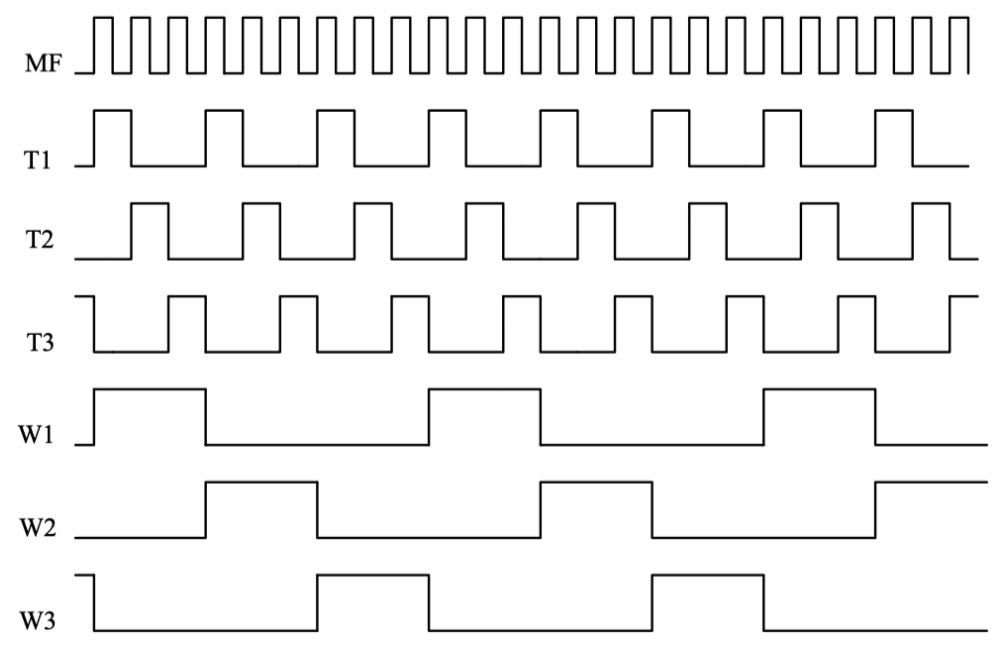
\includegraphics[width=0.9\linewidth]{figures/chapter1/timing.png}
    \caption{时序信号}
\end{figure}

其中主时钟MF频率为1MHz,T1、T2、T3为节拍脉冲信号,W1~W3为节拍电位信号。时序信号在设计控制器时起到重要作用,W节拍电位信号可以用于标志指令执行阶段,T3脉冲控制内部状态变化。

